\section{Experiments}
\label{sec:Experiments}



\subsection{Experimental Setup and Execution}
\label{sec:sec:experiments}

We use the methodology in Section \ref{sec:Methodology} to compare coverage based test generation with unguided/random test model generation. 

Coverage based test strategies as previously introduced in Section \ref{sec:sec:testStrategy} consist of two test criteria {\AllRanges} and {\AllPartitions}.  These test criteria generate model fragments from an effective input meta-model. A test set satisfying {\AllRanges} must contain test models that contain all consistent model fragments from the {\AllRanges} criteria. Similarly, a test set satisfying {\AllPartitions} must contain all consistent model fragments generated from the {\AllPartitions} criteria.

We generate sets of test models based on factorial experimental design \cite{shari2005}. We consider the \emph{exact number of objects for each class} in the effective input meta-model as factors for experimental design. A factor level is the exact number of objects of a given class in a test model. These factors help study the effect of number of different types of objects on the mutation score. For instance, we can ask questions such as whether a large number of {\Association} objects have a correlation with the mutation score? The large of number {\Association} objects also indicates a highly connected {\UML} class diagram test model. We decide these factor levels by simple experimentation such as verifying if models can be generated in reasonable amount of time given that we need to generate thousands of test models in a few hours. We also want to cover a combination of a large number of varying factor levels. We have 8 different factor levels for the different classes in the {\UML} class diagram effective input meta-model as shown in Table \ref{table:mfFactorsa}. Other factors that may affect but are not considered for test model generation are the use different SAT solvers such as SAT4J, MiniSAT, or ZChaff, maximum time to solve, t-wise interaction between model fragments.

The {\AllRanges} criteria on the {\UMLCD} meta-model gives 15 consistent model fragments (see Table \ref{table:modelFrags}). We have 150 models in a set, where 10 non-isomorphic models satisfies each different model fragment. We generate 10 non-isomorphic models to verify that mutation scores do not drastically change within each solution. We synthesize 8 sets of 150 models using different levels for factors as shown in Table \ref{table:mfFactorsa} (see rows 1,2,3,4,5,6). The total number of models in these 8 sets is 1200. 

The {\AllPartitions} criteria gives 5 consistent model fragments. We have 50 test models in a set, where 10 non-isomorphic test models satisfies a different model fragment. We synthesize 8 sets of 50 models using factor levels shown in Table \ref{table:mfFactorsa}. The levels for factors for {\AllRanges} and {\AllPartitions} are the same. Total number of models in the 8 sets is 400. The selection of these factors at the moment is not based on a problem-independent strategy. 

We compare test sets generated using {\AllRanges} and {\AllPartitions} with unguided test sets. For each test set of coverage based strategies we generate an equal number of random/unguided models as a reference to qualify the efficiency of different strategies. Precisely, we have 8 sets of 150 unguided test models to compare with {\AllRanges} and 8 sets of 50 unguided test models to compare with {\AllPartitions}. We use the factor levels in Table \ref{table:mfFactorsa}.

\begin{table}

\caption{Factors and their Levels for  Test Sets}
\label{table:mfFactorsa}
\begin{tabular}[a]{p {2 cm}  l  l  l  l  l l  l  l  l}
%& & &\textbf{(a)} & & & & & &
\hline
%				&   &   &   &    & \textbf{Sets}   &    &   &    \\ 
\textbf{Factors} &&  S1 & S2  &  S3 &  S4  &  S5  &  S6  &  S7 &  S8  \\ \hline 
\textbf{\#ClassModel} && 1 & 1 & 1 & 1 & 1 & 1 & 1 & 1 \\ 
\textbf{\#Class}  &&  5 & 5  & 15 & 15 & 5 & 15 & 5 & 15 \\ 
\textbf{\#Association} && 5 & 15 & 5 & 15  & 5  & 5  & 15  & 15 \\  
\textbf{\#Attribute}  && 25 & 25 & 25 & 25 & 30  & 30 & 30 & 30 \\ 
\textbf{\#PrimitiveDataType} && 4 & 4 & 4 & 4 & 4 & 4 & 4 & 4 \\ 
\textbf{Bit-width Integer}  && 5 & 5 & 5 & 5 & 5 & 5 & 5 & 5\\ 
\textbf{\#Models/Set} {\AllRanges} && 15 & 15 & 15 & 15 & 15 & 15 & 15 & 15 \\ 
\textbf{\#Models/Set} {\Unguided} && 15 & 15 & 15 & 15 & 15 & 15 & 15 & 15 \\ 
\textbf{\#Models/Set} {\AllPartitions}  && 5 & 5 & 5 & 5 & 5 & 5 & 5 \\ 
\textbf{\#Models/Set} {\Unguided}  && 5 & 5 & 5 & 5 & 5 & 5 & 5 \\ \hline
\end{tabular}

\end{table}

\begin{table*} 
	%\vspace{-1 cm}
%% increase table row spacing, adjust to taste
\renewcommand{\arraystretch}{1}
\renewcommand{\arrayrulewidth}{1 pt}
\caption{Mutation Scores in Percentage for All Test Model Sets}
\label{table:mutationScores}
\centering
\begin{tabular}{ l  l l l l l l l l }
\hline
\textbf{Set} & 1 & 2 & 3 & 4 & 5 & 6 & 7 & 8\\ \hline
 \textsf{Unguided} \textbf{150 models/set in 8 sets} & 68.56 & 69.9 & 68.04 & 70.1 & 70.1 & 68.55 & 69 & 70.1 \\
 {\AllRanges} \textbf{150 models/set in 8 sets}  &  88.14 & 92.26  &  81.44 & 85 & 91.23 & 80.4 & 91.23 &  88.14 \\ 
 \textsf{Unguided} \textbf{50 models/set in 8 sets} & 70.1 & 62.17 & 68.04 & 70.1 & 65.46 & 68.04 & 69.94 & 70.1 \\ 
{\AllPartitions} \textbf{50 models/set in 8 sets} & 90.72 & 93.3 & 84.53 & 87.62  & 87.62  & 82.98 & 92.78& 88.66 \\ \hline
\end{tabular}

\end{table*}

To summarize, we generate a total of 3200  models using an Intel(R) Core$^{TM}$ 2 Duo processor with  4GB of RAM. We perform mutation analysis of these sets to obtain mutation scores on a grid of 10 Intel Celeron 440 high-end computers. The computation time for generating 3200 models was about 3 hours and mutation analysis took  about 1 week. We discuss the results of mutation analysis in the following section. 

\subsection{Results and Discussion}
\label{sec:results}


Mutation scores for {\AllRanges} test sets are shown in Table \ref{table:mutationScores} (row 2). Mutation scores for test sets obtained using {\AllPartitions} are shown in Table \ref{table:mutationScores} (row 4). We discuss the effects of the influencing factors on the mutation score:
\begin{itemize}
	\item The number of {\Class} objects and {\Association} objects has a strong correlation with the mutation score. There is an increase in mutation score with the level of these factors. This is true for sets from unguided and model fragments based strategies. For instance, the lowest mutation score using {\AllRanges} is 80.41 \%. This corresponds to set 1 where the factor levels are 1,5,5,25,4,5  (see Column for set 1 in Table \ref{table:mfFactorsa}) and highest mutation scores are 91,24 and 92,27\% where the factor levels are 1,15,5,25,4,5 and 1,5,15,25,4,5 respectively  (see Columns for set 3 and set 7 in Table \ref{table:mfFactorsa}).

%	\item We observe a strong correlation of the mutation score with the number of {\Class} and {\Association} objects due to the nature of the injected mutation operators. The  creational, navigational, and filtering mutation operators injected in the model transformation are killed by input test models  using a large number of {\Class} and {\Association} objects. However, we see that unguided models with both large and small number of {\Class} and {\Association} objects are not able to have a mutation score above 70.1\%. There is a clear need for more knowledge to improve this mutation score. 
	\item We observe that {\AllPartitions} test sets containing only 50 models/set gives a score of maximum 93.3\%. The {\AllPartitions} strategy demonstrates that knowledge from two different partitions satisfied by one test model greatly improves bug detecting efficiency. This also opens a new research direction to explore: Finding strategies to combine model fragments to guide generation of  smaller sets of complex test models with better bug detecting effectiveness.
\end{itemize}

We compare unguided test sets with model fragment guided sets in the \emph{box-whisker} diagram shown in Figure \ref{fig:whisker}. The box whisker diagram is useful to visualize groups of numerical data such as mutation scores for test sets. Each box in the diagram is divided into lower quartile (25\%), median, upper quartile (75\% and above), and largest observation and contains statistically significant values. A box may also indicate which observations, if any, might be considered outliers or whiskers. In the box whisker diagram of Figure \ref{fig:whisker} we shown 4 boxes with whiskers for unguided sets and sets for {\AllRanges} and {\AllPartitions}. The X-axis of this plot represents the strategy used to select sets of test models and the Y-axis represents the mutation score for the sets.

\begin{figure*} 

\begin{center}
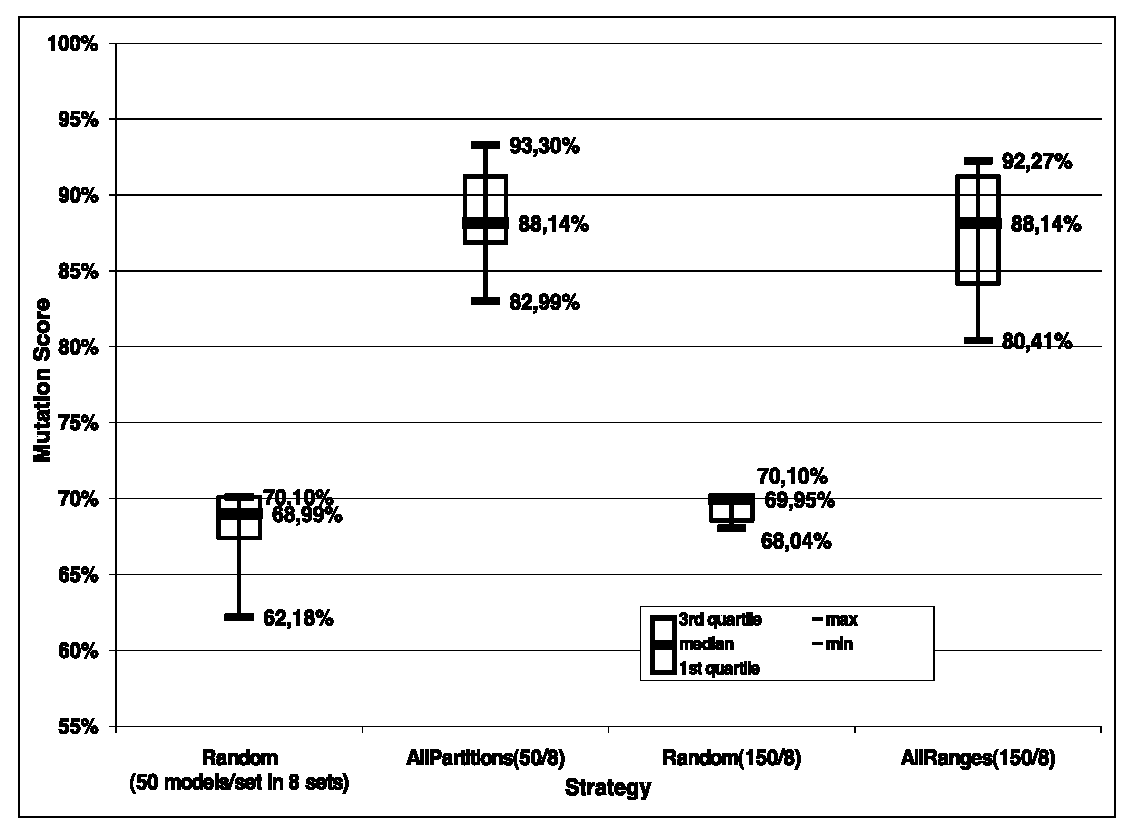
\includegraphics[width=5 in]{./figures/boxplot.eps}
\end{center}
\caption{Box-whisker Diagram to Compare Automatic Model Generation Strategies}
\label{fig:whisker}

\end{figure*}


We make the following observations from the box-whisker diagram:
\begin{itemize}
	\item Both the boxes of {\AllRanges} and {\AllPartitions} represent mutation scores higher than corresponding unguided sets.
	\item The high median mutation scores for strategies {\AllRanges} 88.14\% and {\AllPartitions} 88.14\% indicate that both these strategies return consistently good test sets.
	\item The small size of the box for {\AllPartitions} compared to the {\AllRanges} box indicates its relative convergence to good sets of test models.
	\item The small set of 50 models using {\AllPartitions} gives mutations scores equal or greater than 150 models/set using {\AllRanges}. This implies that it is a more efficient strategy for test model selection. The main consequence is a reduced effort to write corresponding \emph{test oracles} \cite{mottu2008} with 50 models compared to 150 models.
	\item Despite the generation of multiple solutions (10 solutions  for each model fragment or an empty fragment for unguided generation) for each strategy we see a consistent behaviour in the mutation scores. There is no large difference in the mutation scores especially for unguided generation. The median is 69\% and the mutation scores range between 68\% and 70\%. The {\AllRanges} and {\AllPartitions} vary a little more in their mutation scores due to a larger coverage of the effective input meta-model.
\end{itemize}	

The freely and automatically obtained knowledge from the input meta-model using the MMCC algorithm shows that  {\AllRanges} and {\AllPartitions} are successful strategies to guide test generation. They have higher mutation scores with the same sources of knowledge used to generate unguided test sets. A manual analysis of the test models reveals that injection of inheritance via the parent relation in model fragments results in higher mutation scores. Most unguided  models do not contain inheritance relationships as it is not imposed by the meta-model.
 
 What about the 7\% of the mutants that remain alive given that the highest mutation score is 93.3\%? We note by an analysis of the live mutants that they are the same for both {\AllRanges} and {\AllPartitions}. There remain 19 live mutants in a total of 200 injected
mutants (with 6 equivalent mutants). In the median case both AllRanges and AllPartitions strategy give a mutation score of 88.14\%. The live mutants in the median case are mutants not killed due to fewer objects in models.

To consistently achieve a higher mutation score we need more CPU speed, memory and parallelization to efficiently generate larger test models and perform mutation analysis on them. This extension of our work has not be been explored in the paper. It is important for us to remark that some live mutants can only be killed with more information about the model transformation such as those derived from its requirements specification. For instance, one of the remaining live mutant requires a test model with a class containing several primitive type attributes such that at least one is a primary attribute. A test model that satisfies such a requirement requires the combination of model fragments imposing the need for several attributes in a class A, attributes of class A must have  primitive types, at least one primary attribute in the class A, and at least one non-primary attribute in the class A. This requirement can either be specified by manually creating a combination of fragments or by developing a better general test strategy to combine multiple model fragments. In another situation, we observe that not all model fragments are consistent with the input domain and hence they do not really cover the entire meta-model. Therefore, we miss killing some mutants. This information could help improve partitioning and combination strategies to generate better test sets.

